\par Le membre du groupe en charge de cette partie était Antoine Pietri.
\vspace{1cm}
\par Dès le début du projet, nous souhaitions donner à l'analyse de la musique un rôle central dans notre jeu.
Nous avons, en plusieurs étapes, progressé vers un jeu (et ce en particulier dans le mode libre) où la musique
dynamise entièrement le jeu.

\subsubsection{Utilisation de FMOD}

La première chose dont nous avions besoin pour débuter dans l'analyse de la musique était une bibliothèque
qui nous permettait d'accéder aux données d'onde. Nous avons choisi FMOD, qui fournit un adaptateur (ou « wrapper ») en C\#. Puis, il a fallu que nous développions notre propre surcouche de l'API de FMOD qui répondait à nos attentes
(jouer de la musique, récupérer des données de la fonction d'onde, \ldots).

\subsubsection{Spectre sonore}

Une des premières avancées de l'analyse musicale a été l'ajout de la visualisation d'un spectre sonore.
Pour se faire, nous nous sommes servis de la fonction GetSpectrum() fournie par FMOD qui nous donne toutes les
25 ms la liste des amplitudes pour chacune des fréquences.
Le spectre et les infos sonores sont toujours visibles en jeu en appuyant sur F1 :

\begin{center}
	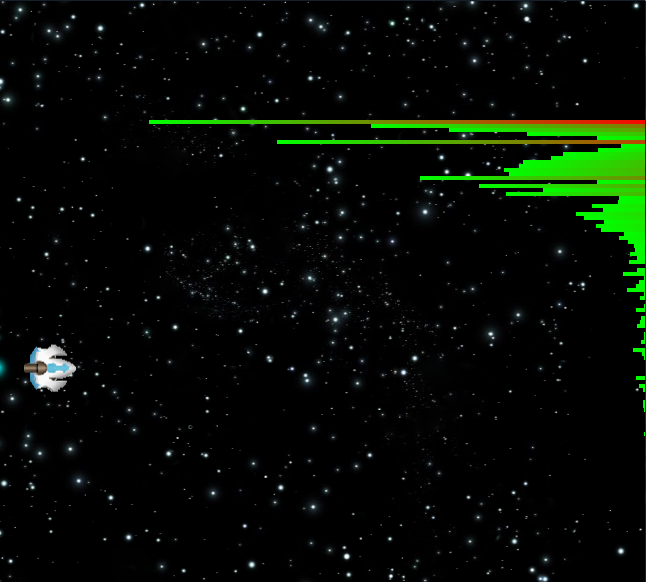
\includegraphics[width=8cm]{images/spectre.png}
\end{center}

\subsubsection{Récupération de l'énergie musicale}
Nous avons ensuite trouvé comment extraire, à partir des amplitudes des données d'onde, l'\emph{énergie} de la musique à un instant précis.
FMOD nous permet d'obtenir un tableau de $2^k$ amplitudes correspondant chacune à une fréquence de chaque sortie audio toutes les 25 millièmes de secondes. Pour obtenir l'énergie de la musique, nous utilisons la formule suivante :
$$E_t = \sqrt{\sum_{i=0}^{2^k - 1} A\footnotesize{\texttt{Left}}_i(t)^2 + A\footnotesize{\texttt{Right}}_i(t)^2}$$
Cependant, comme nous ne faisons pas de distinction des sorties (Stéréo), la formule se simplifie ainsi :
$$E_t = \sum_{i=0}^{2^k - 1} A_i(t)$$

Cette énergie nous sert pour régler la vitesse du fond défilant mais aussi pour moduler la taille des particules
derrière le moteur du vaisseau du joueur.

\subsubsection{Détection de battements : algorithme de base}

\par Pour implémenter le mode Libre, nous avions besoin de détecter les \emph{battements} de la musique choisie par l'utilisateur, et nous avons effectué beaucoup de recherches sur la détection de battements.

\par Pour la troisième soutenance, nous vous avions présenté une version de l'algorithme de détection de battements déjà fonctionnelle, qui a cependant été optimisée depuis.
	
\par Simuler un phénomène physique qui obéit à des équations mathématiques connues est, avec un certain nombre d'approximations, toujours faisable. Mais les concepts plus abstraits, comme les sensations, qui n'obéissent à aucune loi sont souvent bien plus complexes à capturer dans un programme. Le ressenti des battements lors de l'écoute d'une musique est par exemple un phénomène naturel inné chez l'homme. Cependant il existe un certain nombre d'algorithmes qui essaient de s'approcher de manière plus ou moins précise de la détection de battements, dont des approches statistiques que nous avons employé.
\par Plus le son transporte d'énergie, plus il sera perçu fortement. Mais un son sera entendu comme un \emph{battement} seulement si son énergie est largement supérieure à l'énergie moyenne dans un intervalle de temps, c'est à dire si le cerveau détecte une variation brutale dans l'énergie sonore. Cette analyse nous permet de déterminer ainsi les \emph{pics d'énergie sonore}.

\par Dans notre algorithme, nous détectons les grandes variations sonores en calculant la moyenne de l'énergie sonore du signal sur une seconde (44032 échantillons) et en la comparant à l'énergie sonore instantanée, c'est à dire celle contenue sur 1024 échantillons (soit environ 5 millièmes de seconde).
\par On utilise donc l'algorithme suivant :
\begin{itemize}
	\item À partir des deux canaux d'échantillons $(a_n)$ et $(b_n)$, on calcule l'énergie
	instantanée (avec $i_0$ la position des 1024 échantillons à analyser :
	$$e = \sum_{k=i_0}^{i_0 + 1024} a[k]^2 + b[k]^2$$
	
	\item On calcule la moyenne des énergies dans l'intervalle local à partir de notre
	historique des échantillons $B$ :
	$$\langle E \rangle = \frac{1024}{44100} \times \sum_{i=0}^{44032} B_a[i]^2 + B_b[i]^2$$
	
	\item On met à jour notre buffer d'historique en supprimant les 1024 anciens échantillons
	et en mettant les 1024 nouveaux au début (\emph{shift} du buffer)
	
	\item On compare $e$ à $C \times \langle E \rangle $ où $C$ est une constante qui détermine
	 la sensibilité de l'algorithme pour détecter des battements. Nous avons déterminé que
	 $1,3$ était une très bonne constante pour notre jeu. Si $e > \langle E \rangle \times C$,
	 nous avons détecté un battement !
\end{itemize}


\subsubsection{Quelques optimisations directes}

\par La version de l'algorithme présentée lors de la dernière soutenance était la version de base de l'algorithme,
sa vitesse et ses résultats peuvent être améliorés assez facilement. L'algorithme peut tout d'abord être optimisé en
conservant les différentes valeurs de l'énergie musicale calculée sur 1024 échantillons dans notre "historique"
au lieu des échantillons eux-mêmes, afin de ne plus avoir à calculer la moyenne des énergies sur un buffer de 44100 échantillons
mais seulement celle des énergies instantanées $E$. Ce buffer d'énergie correspond à environ une seconde de musique,
c'est à dire qu'il doit contenir un historique des énergies musicales sur 44032 échantillons (calculés en groupe de 1024)
si la vitesse des échantillons est de 44100 par seconde.

\par On va donc créer un nouveau tableau des énergies $E$, où $E[0]$ va contenir la nouvelle énergie calculée sur les
1024 nouveaux échantillons qui viennent d'être ajoutés dans le buffer et $E[42]$\footnote{Non, ce n'est pas fait exprès.}
les 1024 derniers du buffer. On a donc 43 valeurs d'énergie dans l'historique, chacun calculés sur 1024 échantillons ce qui
fait un historique de 44032 énergies d'échantillons, c'est à dire environ une seconde en temps réel.

\par Notre algorithme devient donc :

\begin{itemize}
	\item On calcule, en utilisant la formule de l'algorithme de base, l'énergie instantanée $e$ des 1024 nouveaux échantillons dans le buffer :
	\item On calcule l'énergie moyenne locale $\langle E \rangle$ avc $E$, l'historique des énergies :
	$$\langle E \rangle = \frac{1}{43} \times \sum_{i=0}^{43} (E[i])^2$$
	
	\item On décale le buffer d'énergies $E$ d'\em{un seul} index vers la droite.
	\item On ajoute la nouvelle énergie instantanée $e$ à $E[0]$
	\item On compare $e$ avec $C \times E$
\end{itemize}

\subsubsection{Détection de sensibilité}

\par Un des autres problèmes de cet algorithme « de base » est le choix de la constante $C$. Nous avions vu que 1,3 une bonne valeur pour
l'utilisation que nous en faisions, pourtant elle varie en fonction du style de la musique. Nous devons pallier le fait que notre
algorithme ne peut pas reconnaître les différents instruments : par exemple, une musique de techno ou de rap est assez marquée par
les différents battements (où un choix de $C = 1,4$ pourrait être justifié), bien plus précisément que pour le Rock'N'Roll qui contiennent beaucoup de « bruit », les battements
sont moins marqués et la constante $C$ devrait être plus basse (environ $1,1$).

\par Il nous a donc fallu trouver un moyen de faire en sorte que l'algorithme détermine automatiquement une bonne valeur pour $C$.
Pour cela, nous calculons la variation des énergies contenues dans le buffer d'historique $E$.
Cette variance n'est en fait rien d'autre que la différence $V = E - \langle E \rangle$. Dans notre cas, nous avons donc :

$$V = \frac{1}{43} \times \sum_{i=0}^{43} (E[i] - \langle E \rangle)^2$$

\par Plus cette variance est élevée, plus l'algorithme devrait être sensible, et donc plus $C$ devrait être basse.
Nous allons donc utiliser une fonction affine décroissante pour calculer $C(V)$.

\par Frédéric Patin, auteur de \emph{Beat Detection Algorithms}, a déterminé cette fonction en utilisant des « points » testés pour plusieurs chansons :
$$
C(200) = 1.0\\
C(25) = 1.45\\
$$

\par Nous obtenons donc la fonction décroissante suivante :

$$C = (-0.0025714 \times V) + 1.5142857$$.

\subsubsection{Résultats}
\par Les résultats obtenus sont bien plus efficaces qu'avec la version précédente de l'algorithme. Les battements sont détectés de manière
bien moins approximative que lors de la précédente soutenance. Ils ont été testés avec plusieurs types de musiques,
parmi lesquelles : pop, rock, metal, techno, rap, classique, punk. Encore une fois, les résultats sont extrêmement précis et
semblent juste pour la techno et le rap. Pourtant il arrive que l'algorithme soit parfois trop approximatif pour des musiques
contenant plus de bruit.

\par Détecter des battements est extrêmement frustrant. Nous entendons naturellement ces battements et il nous est très difficile
de les formaliser. Nous avons essayé d'approximer plus ou moins efficacement cette détection, mais le rendu n'est pas
toujours parfait. Cependant, le problème que nous cherchions à résoudre avec cet algorithme, à savoir faire interagir notre perception
du son et celle du jeu, est bien résolu. Les autres méthodes de détection de battement,
passant par le calcul de FFT\footnote{Fast Fourier Transform} sont bien trop lentes (après quelques expériences, il nous a 
fallu plus de 5 minutes pour analyser une musique de 2 minutes 30) pour être utilisées efficacement ici, et l'algorithme expliqué ici
répond parfaitement à nos attentes.

\subsubsection{Le mode libre}

\par Le mode libre est l'application de l'algorithme de détection des battements dans le jeu. Le principe est de générer des niveaux en fonction de la musique analysée.
\par Le jeu commence par construire une \emph{Beat Line}, c'est à dire la liste des différents battements dans le temps. Ensuite, il va calculer la moyenne de toutes les énergies des échantillons de la musique, notée $\langle M \rangle$. Ensuite, à chaque battement détecté à un instant t, le jeu calcule le ratio entre la moyenne locale $\langle E_t \rangle$ et $\langle M \rangle$. Selon les valeurs de ce ratio $r = \frac{\langle E_t \rangle}{\langle M \rangle}$, différents ennemis ou bonus apparaîtrons (le principe étant que plus la musique est forte à cet instant de la partie, plus les ennemis seront puissants).
\par Le positionnement des vaisseaux se fait de manière aléatoire. Cependant, nous avons souhaité que les niveaux générés par des musiques soient uniques, c'est pourquoi le générateur aléatoire est \emph{salé} avec le hash MD5 du contenu du fichier audio intégral.

